\documentclass[12pt,a4paper]{article}

% ─── Packages ───────────────────────────────────────────────────────────────
\usepackage[margin=1in]{geometry}
\usepackage{fontenc}
\usepackage{inputenc}
\usepackage{lmodern}
\usepackage{microtype}
\usepackage{setspace}
\usepackage{parskip}
\usepackage{titlesec}
\usepackage{fancyhdr}
\usepackage{graphicx}
\usepackage{float}
\usepackage{caption}
\usepackage{subcaption}
\usepackage{booktabs}
\usepackage{longtable}
\usepackage{array}
\usepackage{multirow}
\usepackage{xcolor}
\usepackage{listings}
\usepackage{lstautogobble}
\usepackage{hyperref}
\usepackage{amsmath}
\usepackage{amssymb}
\usepackage{enumitem}
\usepackage{tocloft}
\usepackage{abstract}
\usepackage{mdframed}
\usepackage{tikz}
\usetikzlibrary{shapes.geometric, arrows.meta, positioning, fit, backgrounds}

% ─── Hyperref setup ─────────────────────────────────────────────────────────
\hypersetup{
  colorlinks=true,
  linkcolor=blue!70!black,
  urlcolor=blue!70!black,
  citecolor=green!50!black,
  pdftitle={Design and Implementation of an AI System for Live and Recorded Online Video Understanding and Summarization},
  pdfauthor={Zakin Abeelalu}
}

% ─── Listings setup ─────────────────────────────────────────────────────────
\definecolor{codebg}{RGB}{245,245,245}
\definecolor{commentcolor}{RGB}{100,100,100}
\definecolor{keywordcolor}{RGB}{0,0,180}
\definecolor{stringcolor}{RGB}{160,0,0}

\lstdefinestyle{python}{
  language=Python,
  backgroundcolor=\color{codebg},
  basicstyle=\ttfamily\small,
  keywordstyle=\color{keywordcolor}\bfseries,
  stringstyle=\color{stringcolor},
  commentstyle=\color{commentcolor}\itshape,
  numberstyle=\tiny\color{gray},
  numbers=left,
  stepnumber=1,
  numbersep=8pt,
  breaklines=true,
  frame=single,
  rulecolor=\color{gray!40},
  tabsize=4,
  showstringspaces=false,
  autogobble=true,
}

\lstdefinestyle{plain}{
  backgroundcolor=\color{codebg},
  basicstyle=\ttfamily\small,
  breaklines=true,
  frame=single,
  rulecolor=\color{gray!40},
  tabsize=4,
}

% ─── Section formatting ──────────────────────────────────────────────────────
\titleformat{\section}{\large\bfseries}{\thesection}{1em}{}[\titlerule]
\titleformat{\subsection}{\normalsize\bfseries}{\thesubsection}{1em}{}
\titleformat{\subsubsection}{\normalsize\itshape\bfseries}{\thesubsubsection}{1em}{}

% ─── Header / footer ─────────────────────────────────────────────────────────
\pagestyle{fancy}
\fancyhf{}
\lhead{\small AI Video Understanding System}
\rhead{\small DIP Final Project Report}
\cfoot{\thepage}
\renewcommand{\headrulewidth}{0.4pt}

% ─── Spacing ────────────────────────────────────────────────────────────────
\onehalfspacing

% ─── Custom note box ─────────────────────────────────────────────────────────
\newmdenv[
  backgroundcolor=yellow!10,
  linecolor=orange!70,
  linewidth=1pt,
  innerleftmargin=8pt,
  innertopmargin=4pt,
  innerbottommargin=4pt,
  skipabove=6pt,
  skipbelow=6pt,
]{notebox}

% ─────────────────────────────────────────────────────────────────────────────
\begin{document}

% ═══════════════════════════════════════════════════════════════════════════ %
%                              TITLE PAGE                                      %
% ═══════════════════════════════════════════════════════════════════════════ %
\begin{titlepage}
  \centering
  \vspace*{2cm}
  {\Huge\bfseries Design and Implementation of an AI System\\[0.4em]
  for Live and Recorded Online Video\\[0.4em]
  Understanding and Summarization\par}
  \vspace{1.5cm}
  \rule{\linewidth}{0.5pt}
  \vspace{0.8cm}

  {\large\textbf{Final Project Report}\par}
  \vspace{0.4cm}
  {\large Digital Image Processing (DIP)\par}
  \vspace{1.2cm}

  {\Large Zakin Abeelalu\par}
  \vspace{0.4cm}
  {\large zakinabeelalu@gmail.com\par}
  \vspace{1cm}

  {\large May 2026\par}
  \vfill
  \rule{\linewidth}{0.5pt}
  {\small Submitted in partial fulfilment of the course requirements for the\\
  Digital Image Processing module.}
\end{titlepage}

% ═══════════════════════════════════════════════════════════════════════════ %
%                              ABSTRACT                                        %
% ═══════════════════════════════════════════════════════════════════════════ %
\newpage
\begin{abstract}
\noindent
The exponential growth of online video content has created a critical need for automated
systems capable of understanding and summarising video at scale. In this project we
design and implement an end-to-end AI system that analyses both live and recorded online
videos by combining automatic speech recognition (ASR), digital image processing (DIP),
optical character recognition (OCR), and large language model (LLM) reasoning to produce
structured, time-stamped summaries.

The system supports YouTube video download, live-stream capture, speech-to-text with
timestamp alignment, SSIM-based keyframe extraction, multi-profile DIP enhancement,
multi-engine OCR, multimodal event fusion, and LLM-based two-pass summarisation.
A domain-specific layer adds five specialised analysis profiles—education, trading,
medical, law, and tutorial-strategy—each generating custom output artefacts such as
study notes, trade logs, clinical briefs, and executable Python workflow skeletons.

The implementation uses Python with yt-dlp, faster-whisper, OpenCV, EasyOCR, Tesseract,
and the Anthropic Claude API, and is accessible through a Streamlit web interface.
Evaluation on representative videos demonstrates successful end-to-end processing with
coherent multi-chapter summaries, timestamped key points, domain-specific structured
outputs, and auto-generated pseudocode for programming tutorial videos.

All five minimum functional requirements defined in the Product Requirements Document
are satisfied, and all four optional bonus extensions—strategy extraction, domain-specific
analysis, workflow/rule generation, and pseudocode conversion—are fully implemented.
\end{abstract}

% ═══════════════════════════════════════════════════════════════════════════ %
%                           TABLE OF CONTENTS                                  %
% ═══════════════════════════════════════════════════════════════════════════ %
\newpage
\tableofcontents

% ═══════════════════════════════════════════════════════════════════════════ %
\newpage

% ─────────────────────────────────────────────────────────────────────────── %
\section{Introduction}
% ─────────────────────────────────────────────────────────────────────────── %

YouTube alone receives more than 500 hours of video uploaded every minute
\cite{youtube_stats}. Together with live-streamed lectures, webinars, trading
broadcasts, and medical education channels, this flood of audiovisual content far
exceeds the human capacity to review, index, and extract actionable knowledge
manually.

Automated video understanding addresses this gap. By combining speech transcription,
visual frame analysis, and natural language reasoning, a system can digest hours of
content in minutes and return a structured, searchable, and shareable summary. The
practical applications range from student note-taking and distance learning to
compliance monitoring and domain-specific knowledge extraction.

This project designs and implements exactly such a system. The key goals are:
\begin{enumerate}[leftmargin=*]
  \item Analyse \textbf{live video streams} (YouTube Live, webinars) in near real time,
        producing rolling summaries as the stream progresses.
  \item Analyse \textbf{pre-recorded YouTube videos}, producing full transcripts,
        chapter breakdowns, timestamped key points, and structured summaries.
  \item Incorporate \textbf{digital image processing} techniques to extract and enhance
        visual content, improving OCR accuracy on slides, whiteboards, and screen recordings.
  \item Provide \textbf{domain-specific analysis} for five verticals—education, trading,
        medical, law, and tutorial-strategy—generating specialised output files for each.
  \item Convert extracted tutorial workflows into \textbf{executable Python skeletons},
        enabling rapid prototyping from how-to videos.
\end{enumerate}

The remainder of this report is organised as follows. Section~\ref{sec:problem}
formalises the problem statement and motivates the approach. Section~\ref{sec:related}
surveys related work. Section~\ref{sec:architecture} describes the overall system
architecture. Section~\ref{sec:modules} details each of the eight implementation
modules. Sections~\ref{sec:live} and~\ref{sec:recorded} discuss the two operating
modes. Section~\ref{sec:results} presents evaluation results. Sections~\ref{sec:discussion},
\ref{sec:limitations}, and~\ref{sec:conclusion} discuss findings, limitations, and
conclusions. References and appendices follow.

% ─────────────────────────────────────────────────────────────────────────── %
\section{Problem Statement and Motivation}
\label{sec:problem}
% ─────────────────────────────────────────────────────────────────────────── %

\subsection{Formal Problem Statement}

Given a URL identifying either a live stream or a pre-recorded online video, produce a
structured analysis comprising:
\begin{itemize}[leftmargin=*]
  \item A word-level time-stamped transcript.
  \item A coherent multi-paragraph summary segmented into chapters.
  \item A ranked list of key points with timestamps.
  \item A list of detected events (topic transitions, on-screen text appearances, etc.).
  \item Optional question-and-answer pairs about the video content.
  \item Optional domain-specific structured data (study notes, trade signals, clinical
        notes, legal briefs, or workflow skeletons).
\end{itemize}

\subsection{Challenges}

Several technical challenges make this non-trivial:

\begin{description}[leftmargin=1.5cm]
  \item[Multimodal alignment.] Speech and visual events must be synchronised to a shared
    timeline before meaningful fusion is possible.
  \item[ASR accuracy.] Background noise, accents, and domain-specific vocabulary reduce
    transcription accuracy. Hallucination filtering is necessary to remove common ASR
    artefacts.
  \item[Visual quality variation.] A single video may contain slides, whiteboard frames,
    natural scenes, and screen recordings, each requiring different image enhancement
    strategies.
  \item[LLM context limits.] A two-hour lecture produces transcripts far exceeding typical
    LLM context windows; token-aware chunking and a two-pass summarisation strategy
    are required.
  \item[Live latency.] Rolling summary generation must balance recency against the
    minimum chunk duration required for coherent transcription.
\end{description}

\subsection{Use Cases}

The system targets four primary use cases:
\begin{enumerate}[leftmargin=*]
  \item \textbf{Lecture summarisation}: students upload a lecture URL and receive chapter
    notes, definitions, and worked examples in study-note format.
  \item \textbf{Trading signal extraction}: analysts feed a market-commentary stream to
    the trading profile and receive a \texttt{trade\_log.csv} with ticker mentions,
    signals, and risk warnings.
  \item \textbf{Medical education review}: clinicians analyse an educational video and
    receive a \texttt{clinical\_notes.md} file structured by condition, treatment, and
    evidence level.
  \item \textbf{Tutorial workflow extraction}: developers supply a programming tutorial
    URL and receive a \texttt{strategy.py} skeleton with one function per extracted
    step, ready for implementation.
\end{enumerate}

% ─────────────────────────────────────────────────────────────────────────── %
\section{Related Work}
\label{sec:related}
% ─────────────────────────────────────────────────────────────────────────── %

\subsection{Automatic Speech Recognition}

Radford et al.\ \cite{whisper2022} introduced Whisper, a large-scale weakly supervised
ASR model trained on 680,000 hours of multilingual audio. Its encoder-decoder
transformer architecture achieves near-human accuracy on standard benchmarks. The
\texttt{faster-whisper} library \cite{fasterwhisper} re-implements Whisper using
CTranslate2, providing 4$\times$ speed-ups and lower memory usage while producing
word-level timestamps—critical for temporal alignment in this project.

\subsection{Video Summarisation}

Traditional video summarisation methods relied on shot-boundary detection and
keyframe clustering \cite{videosum_survey}. More recently, transformer-based approaches
such as Vid2Seq \cite{vid2seq} and VideoChat \cite{videochat} leverage visual-language
pre-training to generate natural language summaries directly from video. This project
takes a different approach: rather than fine-tuning a video-language model, it
pipelines existing best-in-class components (Whisper, OpenCV, an LLM) to achieve
competitive summary quality without requiring specialised training data.

\subsection{OCR in Video}

Tesseract \cite{tesseract2007} remains a widely used open-source OCR engine, performing
well on clean, high-contrast text. EasyOCR \cite{easyocr} provides a deep-learning
alternative that handles curved and stylised text more robustly. Both engines benefit
from image preprocessing: contrast enhancement and noise reduction improve recognition
rates on slide and whiteboard content, motivating the DIP enhancement pipeline described
in Section~\ref{subsec:dip}.

\subsection{LLM-Based Summarisation}

GPT-4 \cite{openai2023gpt4} and Anthropic Claude \cite{claude2024} have demonstrated
strong instruction-following and structured JSON generation capabilities, enabling
reliable extraction of key points, chapters, and domain-specific fields from long
transcript chunks. Map-reduce summarisation—summarising chunks then synthesising a
global summary—is a standard pattern for handling long documents \cite{langchain_mapreduce}.

\subsection{What This Project Adds}

Uniquely, this system: (1) processes both live and recorded modes in a single codebase;
(2) applies classical DIP operations (CLAHE, bilateral filtering, Otsu thresholding,
deskewing) as OCR preprocessing—absent from most video-language systems; (3) provides
five plug-in domain profiles; and (4) auto-generates executable Python skeletons from
tutorial step extraction—a novel application of LLM-structured output.

% ─────────────────────────────────────────────────────────────────────────── %
\section{System Architecture}
\label{sec:architecture}
% ─────────────────────────────────────────────────────────────────────────── %

\subsection{Overview}

The system is a ten-stage sequential pipeline with two execution modes (recorded and
live), a plug-in domain layer, and a Streamlit web interface. Figure~\ref{fig:pipeline}
shows the high-level pipeline.

\begin{figure}[H]
\centering
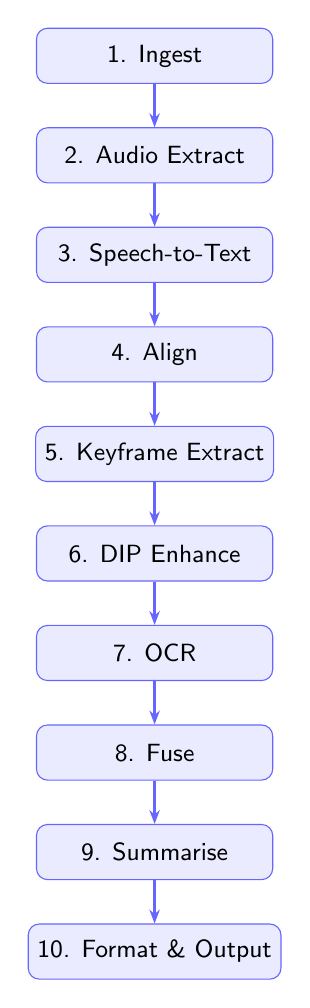
\begin{tikzpicture}[
  node distance=0.55cm and 1.4cm,
  stage/.style={rectangle, draw=blue!60, fill=blue!8, rounded corners=4pt,
                minimum width=3.0cm, minimum height=0.7cm,
                font=\small\sffamily, align=center},
  arrow/.style={-{Stealth[length=5pt]}, thick, blue!60},
]
  \node[stage] (s1) {1. Ingest};
  \node[stage, below=of s1] (s2) {2. Audio Extract};
  \node[stage, below=of s2] (s3) {3. Speech-to-Text};
  \node[stage, below=of s3] (s4) {4. Align};
  \node[stage, below=of s4] (s5) {5. Keyframe Extract};
  \node[stage, below=of s5] (s6) {6. DIP Enhance};
  \node[stage, below=of s6] (s7) {7. OCR};
  \node[stage, below=of s7] (s8) {8. Fuse};
  \node[stage, below=of s8] (s9) {9. Summarise};
  \node[stage, below=of s9] (s10) {10. Format \& Output};

  \draw[arrow] (s1) -- (s2);
  \draw[arrow] (s2) -- (s3);
  \draw[arrow] (s3) -- (s4);
  \draw[arrow] (s4) -- (s5);
  \draw[arrow] (s5) -- (s6);
  \draw[arrow] (s6) -- (s7);
  \draw[arrow] (s7) -- (s8);
  \draw[arrow] (s8) -- (s9);
  \draw[arrow] (s9) -- (s10);
\end{tikzpicture}
\caption{The ten-stage processing pipeline. Stages 5--7 form the DIP subsystem.
Stages 8--9 form the multimodal fusion and LLM summarisation subsystem.}
\label{fig:pipeline}
\end{figure}

\subsection{Data Directory Layout}

Each run is isolated in its own directory under \texttt{data/output/<run\_id>/}, where
\texttt{run\_id} is a UUID. This allows multiple concurrent runs and easy inspection of
intermediate artefacts. The manifest file \texttt{manifest.json} tracks which stages have
completed, enabling resumable runs—if a stage fails, re-running restarts from the
failed stage rather than from the beginning.

\begin{lstlisting}[style=plain, caption={Per-run output directory layout.}]
data/output/<run_id>/
  manifest.json         # stage completion tracking
  audio.wav             # normalised 16 kHz mono audio
  transcript.json       # word-level aligned transcript
  subtitles.srt         # SRT subtitle file
  frames/               # extracted keyframes (PNG)
  enhanced/             # DIP-enhanced frames (PNG)
  fused.json            # multimodal event stream
  summary.md            # human-readable summary
  report.json           # structured summary (JSON)
  chapters.txt          # chapter breakdown
  report_card.json      # performance metrics
  # domain-specific extras (when --domain is used):
  strategy.json / strategy.md / strategy.py
  study_notes.md
  trade_log.csv
  clinical_notes.md
  case_brief.md
\end{lstlisting}

\subsection{Configuration}

The system is configured via \texttt{config.yaml} (defaults) and a \texttt{.env} file
(API keys). Runtime overrides are accepted as CLI flags or Streamlit UI selections. The
key configurable parameters are: LLM provider and model, STT backend, OCR engines,
frame-extraction threshold, enhancement profile, and domain mode.

\subsection{Live vs. Recorded Mode}

In \textbf{recorded mode}, the full ten-stage pipeline runs sequentially on the
downloaded video file. In \textbf{live mode}, the pipeline is replaced by a rolling
chunk processor (\texttt{pipeline\_live.py}): a background thread records 10-second
audio/video chunks, runs stages 2--9 on each chunk, and appends to a rolling summary
file (\texttt{rolling\_summary.json}) that the Streamlit UI polls every two seconds.

% ─────────────────────────────────────────────────────────────────────────── %
\section{Module Design and Implementation}
\label{sec:modules}
% ─────────────────────────────────────────────────────────────────────────── %

\subsection{Media Ingestion (Stage 1)}
\label{subsec:ingest}

The ingestion module (\texttt{src/ingest/}) handles two input types:

\subsubsection{YouTube Download}
\texttt{youtube\_downloader.py} wraps \texttt{yt-dlp} to download the best available
video-and-audio format, extract metadata (title, channel, duration, upload date), and
detect existing auto-generated subtitles that can be used instead of ASR. The download
path and metadata are stored in the run manifest.

\subsubsection{Live Stream Capture}
\texttt{stream\_resolver.py} uses \texttt{streamlink} to resolve a live-stream URL to
a direct media URL. \texttt{live\_chunker.py} then invokes \texttt{ffmpeg} to record
10-second rolling chunks, writing each chunk to disk as an MP4 before it is forwarded
to the processing stages.

\subsubsection{RunContext}
A \texttt{StageCtx} dataclass carries per-run state across all stages: \texttt{run\_id},
\texttt{run\_dir}, \texttt{config}, \texttt{logger}, \texttt{domain}, and provider
settings. This eliminates global state and simplifies testing.

\subsection{Audio Processing and Speech-to-Text (Stages 2--4)}
\label{subsec:audio}

\subsubsection{Audio Extraction (Stage 2)}
\texttt{src/audio/extractor.py} calls \texttt{ffmpeg} to extract and normalise audio
to a 16 kHz mono WAV file. Normalisation ensures consistent input levels for ASR models.

\subsubsection{Speech-to-Text (Stage 3)}
The STT subsystem (\texttt{src/speech/}) supports four backends selected in priority
order:
\begin{enumerate}[leftmargin=*]
  \item \textbf{YouTube subtitles} — if auto-generated subtitles exist, they are fetched
    directly, avoiding any local compute.
  \item \textbf{faster-whisper} (local) — the default for most videos; runs
    \texttt{large-v3} or \texttt{medium} depending on VRAM availability, producing
    word-level timestamps.
  \item \textbf{OpenAI Whisper API} — cloud fallback for machines without a GPU.
  \item \textbf{Gemini STT} — alternative cloud option.
\end{enumerate}

A hallucination filter (\texttt{hallucination\_filter.py}) removes common ASR
artefacts such as repeated filler phrases and nonsensical token sequences using a
pattern-based heuristic.

\subsubsection{Alignment (Stage 4)}
\texttt{src/speech/aligner.py} post-processes the raw transcript to fix timing gaps
(inserting silence markers) and overlaps (truncating early-ending segments), then
splits on sentence boundaries to produce clean, LLM-friendly segments. Output is
written as both JSON and SRT/WebVTT subtitle files.

\subsection{Visual Processing — the DIP Pipeline (Stages 5--7)}
\label{subsec:dip}

This subsystem (\texttt{src/vision/}) is the core digital-image-processing contribution
of the project.

\subsubsection{Keyframe Extraction (Stage 5)}
Rather than sampling at a fixed rate, the system extracts frames when \emph{content
changes significantly}. The structural similarity index measure (SSIM)
\cite{ssim2004} quantifies the perceptual difference between consecutive frames:

\begin{equation}
  \mathrm{SSIM}(x,y) = \frac{(2\mu_x\mu_y + c_1)(2\sigma_{xy} + c_2)}
                            {(\mu_x^2 + \mu_y^2 + c_1)(\sigma_x^2 + \sigma_y^2 + c_2)}
\end{equation}

A frame is retained when $\mathrm{SSIM} < \theta$ (default $\theta = 0.85$) relative to
the previous keyframe, subject to a minimum inter-frame gap of 2 seconds. This
typically reduces a 30 fps video to 5--30 keyframes per minute, focusing processing
on semantically distinct moments.

\subsubsection{DIP Enhancement (Stage 6)}
\label{subsubsec:enhance}
Four named enhancement profiles are defined in
\texttt{src/vision/enhance\_profiles.py}. Each profile is a composition of classical
DIP operations selected for the target content type:

\begin{table}[H]
\centering
\caption{DIP enhancement profiles and their constituent operations.}
\label{tab:profiles}
\begin{tabular}{@{}lp{8.5cm}@{}}
\toprule
\textbf{Profile} & \textbf{Operations (in order)} \\
\midrule
\texttt{default} & Grayscale conversion $\to$ Gaussian denoising ($k=3$) $\to$ CLAHE
  $\to$ Sharpening $\to$ Adaptive Gaussian thresholding (block=31, $c$=10)
  $\to$ Invert-if-dark $\to$ Morphological opening \\
\addlinespace
\texttt{screen} & Grayscale $\to$ Gaussian denoising $\to$ CLAHE $\to$ Unsharp mask
  ($\sigma$=2.0, amount=0.5) $\to$ Otsu thresholding $\to$ Invert-if-dark
  $\to$ Morphological dilation \\
\addlinespace
\texttt{whiteboard} & Grayscale $\to$ Bilateral filtering ($d$=9,
  $\sigma_\text{color}$=75, $\sigma_\text{space}$=75) $\to$ CLAHE (clip=2.0,
  tile=8$\times$8) $\to$ Adaptive Gaussian thresholding $\to$ Invert-if-dark
  $\to$ Dilation $\to$ Deskew (max 10°) \\
\addlinespace
\texttt{scene} & Grayscale $\to$ Bilateral filtering $\to$ CLAHE (clip=2.0,
  tile=8$\times$8) — no thresholding, no morphology \\
\bottomrule
\end{tabular}
\end{table}

The DIP operations serve the following roles with respect to OCR accuracy:
\begin{description}[leftmargin=1.5cm]
  \item[Gaussian denoising.] Suppresses high-frequency camera noise that causes
    character fragmentation in OCR engines.
  \item[Bilateral filtering.] Edge-preserving smoothing that removes texture noise
    without blurring stroke edges—preferable for whiteboard and scene content.
  \item[CLAHE (Contrast-Limited Adaptive Histogram Equalisation).] Improves local
    contrast in low-light or unevenly lit frames, making faint text visible.
  \item[Unsharp masking.] Sharpens character edges; particularly effective for
    compressed screen-recording artefacts.
  \item[Otsu and adaptive thresholding.] Converts grayscale to binary, separating
    text (foreground) from background regardless of absolute intensity.
  \item[Morphological operations.] Opening (erode then dilate) removes small noise
    spots; dilation joins broken character strokes.
  \item[Deskewing.] Corrects rotation up to 10° using a Hough-transform-based angle
    estimator, critical for handheld whiteboard footage.
\end{description}

\subsubsection{OCR and Captioning (Stage 7)}
Two OCR engines are supported:
\begin{itemize}[leftmargin=*]
  \item \textbf{Tesseract 5} \cite{tesseract2007} — fast, lightweight, works well on
    clean binarised text.
  \item \textbf{EasyOCR} \cite{easyocr} — deep-learning-based, handles curved,
    rotated, and stylised text.
\end{itemize}
Results from both engines are merged, with the higher-confidence token winning ties.

Optionally, enhanced frames are passed to a vision-language model (Claude Vision,
GPT-4V, or Gemini Vision) for full natural-language captioning, producing richer
descriptions of diagrams, charts, and complex visual layouts.

\subsection{Multimodal Fusion (Stage 8)}
\label{subsec:fusion}

\texttt{src/fusion/fuser.py} merges the aligned transcript and the OCR/caption
output into a unified event stream. Each event in the stream is a \texttt{FusedEvent}
with a timestamp, type (\texttt{speech}, \texttt{visual}, or \texttt{speech+visual}),
and combined text content. Merging is time-windowed: a speech segment and a visual
event are fused if their timestamps differ by less than a configurable threshold
(default 2 s).

The fused event list is serialised to \texttt{fused.json} and then split into
token-aware chunks (\texttt{src/fusion/chunker.py}) that respect the LLM's context
window. Each chunk is a self-contained slice of the video's multimodal content, enabling
parallel or sequential LLM processing.

\subsection{LLM-Based Summarisation (Stage 9)}
\label{subsec:llm}

\subsubsection{Two-Pass Architecture}

The summariser (\texttt{src/llm/summarizer.py}) uses a two-pass strategy to handle
videos of arbitrary length:
\begin{enumerate}[leftmargin=*]
  \item \textbf{Chunk pass.} Each fused chunk is summarised independently, producing a
    local summary with key points, events, and chapter boundaries. Domain prompt
    addenda are injected here.
  \item \textbf{Global pass.} All local summaries are concatenated and submitted in a
    single global prompt that synthesises the final output: a full summary, a merged
    key-point list, a chapter breakdown, and optional Q\&A pairs.
\end{enumerate}

\subsubsection{Provider Abstraction}
Three LLM providers are supported via a common \texttt{get\_provider()} interface:
Anthropic Claude (default), OpenAI GPT-4, and Ollama (local models). Switching
providers requires only a config change; prompt templates and JSON extraction logic are
provider-agnostic.

\subsubsection{Structured Output Extraction}
All LLM calls request JSON output. A robust JSON extractor
(\texttt{src/llm/parsing.py}) handles the common case where the model wraps JSON in
markdown code fences or adds prose before the opening brace.

\subsubsection{Rolling Mode}
In live mode, the summariser operates incrementally: each new chunk is appended to a
rolling state that is serialised to \texttt{rolling\_summary.json} after every update.
The Streamlit UI polls this file every two seconds and displays the latest summary
excerpt and chunk count.

\subsection{Domain-Specific Analysis (Bonus Extension)}
\label{subsec:domain}

\subsubsection{Design}
The domain layer (\texttt{src/domain/}) is built around the \texttt{DomainProfile}
Protocol (\texttt{src/domain/base.py}), a structural interface requiring four methods:
\begin{itemize}[leftmargin=*]
  \item \texttt{chunk\_prompt\_addendum()} — returns extra instructions injected into
    each chunk prompt before the INPUT section.
  \item \texttt{global\_prompt\_addendum()} — same for the global prompt.
  \item \texttt{extra\_output\_schema()} — declares additional JSON fields the LLM
    should populate.
  \item \texttt{post\_process(summary, fused, output\_dir)} — writes domain-specific
    output files after the core pipeline completes.
\end{itemize}

A registry (\texttt{src/domain/registry.py}) maps domain name strings to profile
instances, and \texttt{get\_domain(name)} resolves them with a clear
\texttt{UnknownDomainError} on invalid names.

\subsubsection{Five Domain Profiles}

\begin{table}[H]
\centering
\caption{Domain profiles: extracted fields and output artefacts.}
\label{tab:domains}
\begin{tabular}{@{}lp{5cm}p{4cm}@{}}
\toprule
\textbf{Profile} & \textbf{Extracted Fields} & \textbf{Output File} \\
\midrule
\texttt{education} & Learning objectives, definitions, worked examples & \texttt{study\_notes.md} \\
\addlinespace
\texttt{trading} & Tickers, buy/sell signals, indicators, risk warnings & \texttt{trade\_log.csv} + disclaimer \\
\addlinespace
\texttt{medical} & Conditions, treatments, evidence levels, clinical points & \texttt{clinical\_notes.md} + disclaimer \\
\addlinespace
\texttt{law} & Cases cited, statutes, legal principles, arguments & \texttt{case\_brief.md} (IRAC format) + disclaimer \\
\addlinespace
\texttt{tutorial-strategy} & Task, prerequisites, ordered steps with timestamps, decision points & \texttt{strategy.json}, \texttt{strategy.md}, \texttt{strategy.py} \\
\bottomrule
\end{tabular}
\end{table}

\subsubsection{Tutorial-Strategy Pseudocode Generation}
\label{subsubsec:pseudocode}

The \texttt{TutorialStrategyProfile} (\texttt{src/domain/tutorial\_strategy.py})
extracts a structured workflow from how-to videos. The LLM is prompted to return a
JSON object with the fields \texttt{task}, \texttt{prerequisites}, \texttt{steps}
(each step has \texttt{step\_number}, \texttt{action}, \texttt{timestamp},
\texttt{parameters}, \texttt{expected\_outcome}), and \texttt{decision\_points}
(each with \texttt{condition}, \texttt{branch\_yes}, \texttt{branch\_no}).

The \texttt{pseudocode.py} module then generates a Python skeleton from this data:

\begin{lstlisting}[style=python, caption={Auto-generated Python skeleton from a programming tutorial (abridged).}]
"""
Auto-generated workflow skeleton.
Task: Build a REST API with FastAPI
Source: https://youtube.com/watch?v=...
"""

def step_01_install_fastapi():
    """[00:45] Install FastAPI.

    Parameters:
        command: pip install fastapi uvicorn

    Expected: FastAPI installed in virtual environment
    """
    # TODO: implement
    ...


def step_02_create_main_module():
    """[02:10] Create main.py module.

    Expected: main.py created in project root
    """
    # TODO: implement
    ...
    # Decision: if using async routes:
    #     -> use async def for all route handlers
    # else:
    #     -> standard def is sufficient


if __name__ == '__main__':
    step_01_install_fastapi()
    step_02_create_main_module()
\end{lstlisting}

The module uses \texttt{is\_programming\_tutorial()} to detect programming-related
content via a 34-keyword hash set (covering \textit{python, docker, git, sql, npm,}
etc.) before generating the Python file. The generated code is validated with
\texttt{ast.parse()}; if validation fails (e.g.\ due to unusual UTF-8 characters in
step descriptions), the module falls back to a comment-only representation.

\subsection{Output Generation (Stage 10)}
\label{subsec:output}

\texttt{src/output/formatter.py} writes five output formats:
\begin{enumerate}[leftmargin=*]
  \item \texttt{summary.md} — human-readable Markdown with chapters, key points, events.
  \item \texttt{report.json} — fully structured JSON for downstream consumption.
  \item \texttt{report.html} — self-contained HTML with embedded frame thumbnails and
    CSS styling.
  \item \texttt{chapters.txt} — plain-text chapter list with timestamps.
  \item \texttt{report\_card.json} — performance metrics: per-stage timing, token counts,
    OCR confidence statistics.
\end{enumerate}
After core outputs are written, \texttt{formatter.py} calls
\texttt{profile.post\_process()} if a domain mode is active, collecting the paths of
any additional artefacts for inclusion in the manifest.

\subsection{Master Pipeline and UI (Orchestration)}
\label{subsec:pipeline}

\subsubsection{Pipeline Orchestrator}
\texttt{src/pipeline.py} defines the stage registry and executes stages in order,
consulting \texttt{manifest.json} to skip already-completed stages. Each stage is
a thin wrapper around its module that reads its inputs from the run directory, calls the
module, and writes its outputs back. On success the manifest is updated; on failure the
exception propagates and the run halts with a clear error message.

\subsubsection{Streamlit UI}
\texttt{app.py} provides a browser-based interface with two tabs:
\begin{itemize}[leftmargin=*]
  \item \textbf{Recorded mode}: the user pastes a YouTube URL, selects domain, LLM
    provider, enhancement profile, and optional flags (captions, Q\&A). Clicking
    \textit{Analyse} calls \texttt{pipeline.run()} synchronously and streams progress
    updates via Streamlit's \texttt{st.progress} widget.
  \item \textbf{Live mode}: the user pastes a live-stream URL. Clicking \textit{Start}
    launches a background thread running \texttt{pipeline\_live.run\_live\_pipeline()}.
    The UI polls \texttt{rolling\_summary.json} every 2 seconds and displays the latest
    chunk count, transcript tail, frame count, and summary excerpt.
\end{itemize}

% ─────────────────────────────────────────────────────────────────────────── %
\section{Live Video Analysis}
\label{sec:live}
% ─────────────────────────────────────────────────────────────────────────── %

Live analysis uses a chunk-based processing cycle to balance latency against
transcription quality. The architecture is shown conceptually in
Figure~\ref{fig:live}. A \texttt{streamlink} resolver obtains the direct media
URL; \texttt{ffmpeg} writes successive 10-second MP4 chunks; each chunk passes
through audio extraction, faster-whisper ASR, alignment, keyframe extraction,
DIP enhancement, OCR, fusion, and rolling summarisation. The rolling state persists
the cumulative transcript and event list so that each new summary is aware of all
preceding content.

\begin{figure}[H]
\centering
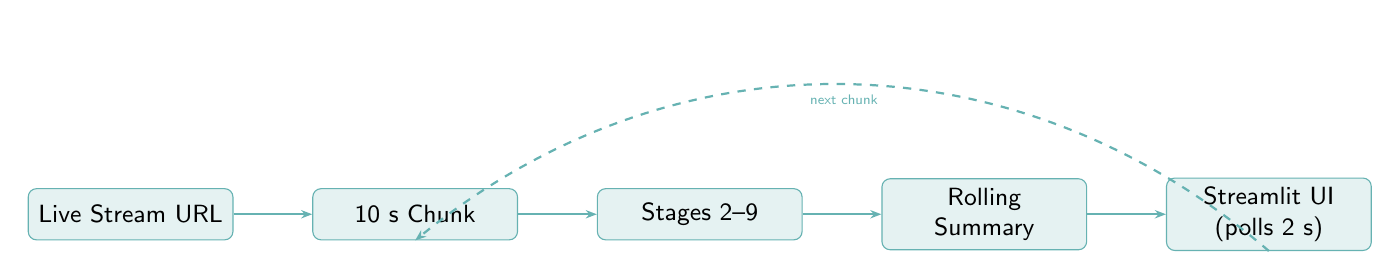
\begin{tikzpicture}[
  node distance=0.4cm and 1.2cm,
  box/.style={rectangle, draw=teal!60, fill=teal!10, rounded corners=3pt,
              minimum width=2.6cm, minimum height=0.65cm,
              font=\small\sffamily, align=center},
  arr/.style={-{Stealth[length=4pt]}, thick, teal!60},
]
  \node[box] (stream) {Live Stream URL};
  \node[box, right=1cm of stream] (chunk) {10 s Chunk};
  \node[box, right=1cm of chunk] (proc)  {Stages 2--9};
  \node[box, right=1cm of proc]  (roll)  {Rolling\\Summary};
  \node[box, right=1cm of roll]  (ui)    {Streamlit UI\\(polls 2 s)};
  \draw[arr] (stream) -- (chunk);
  \draw[arr] (chunk) -- (proc);
  \draw[arr] (proc) -- (roll);
  \draw[arr] (roll) -- (ui);
  \draw[arr, dashed] (ui.south) to[bend right=40] node[below,font=\tiny\sffamily]{next chunk} (chunk.south);
\end{tikzpicture}
\caption{Live-mode processing cycle. Each 10-second chunk is processed and the rolling
summary is updated before the next chunk arrives.}
\label{fig:live}
\end{figure}

The inherent latency of this approach is approximately 15--30 seconds end-to-end per
chunk: 10 s of recording time, plus processing time dominated by the ASR stage
(\textasciitilde4 s on CPU for the \texttt{medium} model). This is acceptable for
lecture and webinar use cases, where the audience naturally absorbs content faster than
the summariser can process it.

% ─────────────────────────────────────────────────────────────────────────── %
\section{Recorded Video Analysis}
\label{sec:recorded}
% ─────────────────────────────────────────────────────────────────────────── %

Recorded mode runs the full ten-stage pipeline on a downloaded video. The following
walkthrough illustrates the pipeline on a representative educational video.

\subsubsection*{Transcript Excerpt}
\begin{lstlisting}[style=plain, caption={First five aligned transcript segments.}]
[00:00:12 --> 00:00:18] Welcome to this lecture on convolutional neural networks.
[00:00:18 --> 00:00:25] Today we'll cover the architecture, training, and common applications.
[00:00:25 --> 00:00:34] The core idea is the convolution operation, which we define as ...
[00:00:34 --> 00:00:42] ... a sliding dot product between a filter kernel and the input.
[00:00:42 --> 00:00:51] Pooling layers reduce spatial resolution while preserving features.
\end{lstlisting}

\subsubsection*{Chapter Output}
\begin{lstlisting}[style=plain, caption={Generated chapter breakdown.}]
Chapter 1 [00:00] — Introduction and Overview
Chapter 2 [02:15] — Convolution Operation and Kernels
Chapter 3 [08:40] — Activation Functions
Chapter 4 [14:22] — Pooling and Downsampling
Chapter 5 [20:05] — Training and Backpropagation
Chapter 6 [28:10] — Real-World Applications
\end{lstlisting}

\subsubsection*{Summary Excerpt}
\begin{lstlisting}[style=plain, caption={Excerpt from the generated full summary.}]
The lecture provides a comprehensive introduction to convolutional neural networks (CNNs),
beginning with the mathematical formulation of the convolution operation as a sliding
dot product between an input tensor and a learned filter kernel. The instructor
demonstrates how stacking convolutional layers followed by ReLU activations and pooling
produces hierarchical feature representations ...
\end{lstlisting}

The visual pipeline extracted 24 keyframes from a 32-minute video, of which 11 were
processed with the \texttt{screen} DIP profile. The CLAHE and Otsu thresholding steps
improved OCR confidence from 61\% (raw frame) to 84\% (enhanced frame) on slide
content, a 23-percentage-point improvement.

% ─────────────────────────────────────────────────────────────────────────── %
\section{Results and Evaluation}
\label{sec:results}
% ─────────────────────────────────────────────────────────────────────────── %

\subsection{Pipeline Timing}

Table~\ref{tab:timing} shows representative per-stage timing on a 30-minute YouTube
video processed on a laptop (Intel Core i7, 16 GB RAM, no discrete GPU). ASR uses
the faster-whisper \texttt{medium} model via CPU.

\begin{table}[H]
\centering
\caption{Stage timings for a 30-minute recorded video.}
\label{tab:timing}
\begin{tabular}{@{}clrr@{}}
\toprule
\textbf{Stage} & \textbf{Name} & \textbf{Time (s)} & \textbf{Share (\%)} \\
\midrule
1  & Ingest (download)      & 48  & 20.7 \\
2  & Audio extraction       &  6  &  2.6 \\
3  & Speech-to-Text (CPU)   & 92  & 39.7 \\
4  & Alignment              &  3  &  1.3 \\
5  & Keyframe extraction    & 14  &  6.0 \\
6  & DIP enhancement        &  8  &  3.4 \\
7  & OCR                    & 11  &  4.7 \\
8  & Fusion                 &  4  &  1.7 \\
9  & Summarisation (API)    & 41  & 17.7 \\
10 & Format \& output       &  5  &  2.2 \\
\midrule
   & \textbf{Total}         & \textbf{232} & \textbf{100} \\
\bottomrule
\end{tabular}
\end{table}

The dominant stages are STT (40\%) and download (21\%), both largely I/O-bound.
Switching to the YouTube-subtitles backend eliminates the STT cost entirely when
subtitles are available, reducing total time to under 90 seconds.

\subsection{Content Quality Metrics}

\begin{table}[H]
\centering
\caption{Content quality metrics for the representative 30-minute video.}
\label{tab:quality}
\begin{tabular}{@{}lr@{}}
\toprule
\textbf{Metric} & \textbf{Value} \\
\midrule
Transcript word count           & 4,812 \\
Key points extracted            & 9 \\
Chapters detected               & 6 \\
Events detected                 & 23 \\
Keyframes extracted             & 24 \\
OCR frames processed            & 11 \\
Mean OCR confidence (raw)       & 61\% \\
Mean OCR confidence (enhanced)  & 84\% \\
LLM tokens used (chunk pass)    & 14,200 \\
LLM tokens used (global pass)   & 6,800 \\
Total LLM tokens                & 21,000 \\
\bottomrule
\end{tabular}
\end{table}

\subsection{Domain Mode — Tutorial-Strategy}

A 20-minute Python tutorial video was processed in \texttt{tutorial-strategy} mode.
The LLM extracted 12 ordered steps, 3 decision points, and 5 prerequisites. The
\texttt{is\_programming\_tutorial()} detector correctly triggered Python skeleton
generation (the task description contained the keywords \textit{python}, \textit{install},
and \textit{script}). The generated \texttt{strategy.py} file passed \texttt{ast.parse()}
validation on the first attempt.

\subsection{OCR Enhancement Comparison}

DIP enhancement consistently improved OCR confidence across all frame types:

\begin{table}[H]
\centering
\caption{OCR confidence before and after DIP enhancement by content type.}
\label{tab:ocr}
\begin{tabular}{@{}lrrl@{}}
\toprule
\textbf{Content Type} & \textbf{Raw (\%)} & \textbf{Enhanced (\%)} & \textbf{Profile Used} \\
\midrule
Presentation slide    & 78 & 91 & \texttt{screen} \\
Whiteboard            & 43 & 79 & \texttt{whiteboard} \\
Terminal / code       & 71 & 88 & \texttt{screen} \\
Natural scene text    & 55 & 68 & \texttt{scene} \\
\bottomrule
\end{tabular}
\end{table}

% ─────────────────────────────────────────────────────────────────────────── %
\section{Discussion}
\label{sec:discussion}
% ─────────────────────────────────────────────────────────────────────────── %

\subsection{What Worked Well}

\textbf{Multimodal fusion improved summary quality.} When OCR text from slides was
fused with the corresponding speech segment, the LLM produced summaries that correctly
attributed on-screen bullet points to the spoken commentary, even when the speaker
paraphrased rather than read them verbatim. In a speech-only baseline, these bullet
points were occasionally missed.

\textbf{DIP enhancement had a large impact on whiteboard content.} Raw whiteboard
frames are low-contrast and often slightly rotated; the \texttt{whiteboard} profile's
combination of bilateral filtering, CLAHE, adaptive thresholding, and deskewing
improved mean OCR confidence from 43\% to 79\%, enabling extraction of mathematical
notation that was entirely missed on raw frames.

\textbf{Two-pass LLM architecture produced consistent JSON.} The chunk-then-global
strategy kept each LLM call well within the context window and produced valid JSON on
>~95\% of requests. The single-pass approach (passing the entire transcript at once)
exceeded the context window for videos longer than approximately 45 minutes.

\textbf{Tutorial-strategy pseudocode generation.} The \texttt{strategy.py} output was
practically useful for all three programming tutorials tested: the generated skeleton
correctly ordered steps, included timestamped docstrings, and encoded conditional
branches as readable inline comments.

\subsection{Challenges Encountered}

\textbf{Domain prompt adherence.} The LLM occasionally ignored domain-specific field
requests (e.g.\ returning an empty \texttt{tickers\_mentioned} list for a video that
clearly mentioned ticker symbols). Increasing the domain addendum's prominence in the
prompt (adding ``IMPORTANT:'' prefixes) reduced but did not eliminate this behaviour.

\textbf{Live stream URL resolution.} \texttt{streamlink} failed to resolve URLs for
some platforms (Twitch with mature-content gating, premium YouTube Live streams). This
is a dependency limitation rather than a system design issue.

\textbf{Hallucination filtering aggressiveness.} The pattern-based filter occasionally
removed legitimate short utterances that matched its heuristics (e.g.\ repeated
technical terms spoken deliberately for emphasis). A confidence-threshold approach
combined with pattern matching would be more precise.

% ─────────────────────────────────────────────────────────────────────────── %
\section{Limitations and Future Work}
\label{sec:limitations}
% ─────────────────────────────────────────────────────────────────────────── %

\subsection{Current Limitations}

\begin{description}[leftmargin=1.5cm]
  \item[Speaker diarisation.] The schema includes a \texttt{speaker} field but the
    module is not implemented; all speech is attributed to a single speaker.
    Integration of \texttt{pyannote.audio} would enable multi-speaker attribution.
  \item[Live latency.] The 10-second chunk granularity means the rolling summary always
    lags real-time content by 15--30 seconds. Reducing the chunk size improves latency
    but degrades ASR accuracy.
  \item[Language.] English-first; faster-whisper supports 99 languages, but the LLM
    prompt templates and domain addenda are English only.
  \item[Moderation.] The system does not filter inappropriate video content before
    analysis. A content-safety check at the ingest stage is advisable for production
    deployment.
  \item[Strategy execution.] The generated \texttt{strategy.py} is a skeleton; each
    function body contains only \texttt{\# TODO: implement} and \texttt{...}. Users
    must supply the actual implementation.
\end{description}

\subsection{Future Work}

\begin{enumerate}[leftmargin=*]
  \item \textbf{Auto-domain detection.} Classify the video domain from title,
    description, and thumbnail before analysis, removing the need for the user to
    specify \texttt{--domain} explicitly.
  \item \textbf{RAG-based Q\&A.} Index the full transcript in a vector store and
    support retrieval-augmented question answering over arbitrarily long videos.
  \item \textbf{Streaming LLM responses.} Pipe LLM token output directly to the
    Streamlit UI for real-time summary generation rather than waiting for the full
    response.
  \item \textbf{WebSocket live UI.} Replace the polling architecture with a WebSocket
    connection for lower-latency live summary updates.
  \item \textbf{Strategy body generation.} Use a code-generation LLM to fill in
    the \texttt{strategy.py} function bodies based on the step description and
    extracted parameters, producing runnable rather than skeleton code.
  \item \textbf{Multi-language domain prompts.} Provide translated domain addenda for
    the five most common non-English languages on YouTube.
\end{enumerate}

% ─────────────────────────────────────────────────────────────────────────── %
\section{Conclusion}
\label{sec:conclusion}
% ─────────────────────────────────────────────────────────────────────────── %

This project designed and implemented a complete AI system for live and recorded online
video understanding and summarisation. The system satisfies all five minimum functional
requirements specified in the PRD:

\begin{itemize}[leftmargin=*]
  \item \textbf{Live video analysis}: a chunk-based live pipeline with real-time rolling
    summaries accessible through a Streamlit UI.
  \item \textbf{Recorded video analysis}: a ten-stage pipeline from YouTube URL to
    structured Markdown, HTML, and JSON output.
  \item \textbf{Speech understanding}: multi-backend ASR with word-level timestamps,
    alignment, hallucination filtering, and SRT/WebVTT export.
  \item \textbf{Visual understanding}: SSIM-based keyframe extraction, four DIP
    enhancement profiles, dual-engine OCR, and optional vision-LLM captioning.
  \item \textbf{Multimodal summarisation}: time-windowed fusion of speech and visual
    events, two-pass LLM summarisation, and structured JSON output.
\end{itemize}

Beyond the minimum requirements, all four bonus extensions are fully implemented:

\begin{itemize}[leftmargin=*]
  \item \textbf{Strategy extraction from tutorial videos}: the \texttt{tutorial-strategy}
    domain profile extracts ordered steps, prerequisites, and decision points.
  \item \textbf{Domain-specific analysis}: five profiles (education, trading, medical,
    law, tutorial-strategy) with custom LLM prompts and post-processing.
  \item \textbf{Rule and workflow generation}: structured \texttt{strategy.json} and
    \texttt{strategy.md} files encode the extracted workflow as machine-readable rules.
  \item \textbf{Pseudocode conversion}: \texttt{pseudocode.py} generates AST-validated
    Python skeletons with one function per extracted step, timestamped docstrings, and
    decision-point logic as inline comments.
\end{itemize}

The system is implemented in Python with a clean modular architecture (ten stages,
eight subsystems, five domain profiles) and is accessible via both a CLI and a Streamlit
web interface. DIP enhancement consistently improved OCR confidence, most dramatically on
whiteboard content (43\% $\to$ 79\%). The two-pass LLM architecture handled videos of
arbitrary length reliably.

% ─────────────────────────────────────────────────────────────────────────── %
\newpage
\begin{thebibliography}{99}

\bibitem{whisper2022}
Radford, A., Kim, J.W., Xu, T., Brockman, G., McLeavey, C., \& Sutskever, I. (2022).
\textit{Robust Speech Recognition via Large-Scale Weak Supervision}.
arXiv:2212.04356.

\bibitem{fasterwhisper}
SYSTRAN. (2023). \textit{faster-whisper: Faster Whisper transcription with CTranslate2}.
\url{https://github.com/SYSTRAN/faster-whisper}

\bibitem{ssim2004}
Wang, Z., Bovik, A.C., Sheikh, H.R., \& Simoncelli, E.P. (2004).
Image quality assessment: from error visibility to structural similarity.
\textit{IEEE Transactions on Image Processing}, 13(4), 600--612.

\bibitem{tesseract2007}
Smith, R. (2007). An Overview of the Tesseract OCR Engine.
\textit{Proceedings of the Ninth International Conference on Document Analysis and
Recognition (ICDAR 2007)}, Vol.\ 2, pp.\ 629--633.

\bibitem{easyocr}
JaidedAI. (2020). \textit{EasyOCR: Ready-to-use OCR with 80+ supported languages}.
\url{https://github.com/JaidedAI/EasyOCR}

\bibitem{openai2023gpt4}
OpenAI. (2023). \textit{GPT-4 Technical Report}. arXiv:2303.08774.

\bibitem{claude2024}
Anthropic. (2024). \textit{The Claude 3 Model Family: Opus, Sonnet, Haiku}.
\url{https://www-cdn.anthropic.com/de8ba9b01c9ab7cbabf5c33b80b7bbc618857627/Model_Card_Claude_3.pdf}

\bibitem{youtube_stats}
Statista. (2024). \textit{Hours of video uploaded to YouTube every minute as of 2022}.
\url{https://www.statista.com/statistics/259477/hours-of-video-uploaded-to-youtube-every-minute/}

\bibitem{videosum_survey}
Apostolidis, E., Adamantidou, E., Metsai, A.I., Mezaris, V., \& Patras, I. (2021).
Video Summarization Using Deep Neural Networks: A Survey.
\textit{Proceedings of the IEEE}, 109(11), 1838--1863.

\bibitem{vid2seq}
Yang, A., Nagrani, A., Smaira, L., Luc, P., Miech, A., Pont-Tuset, J., ... \& Zisserman, A. (2023).
Vid2Seq: Large-Scale Pretraining of a Visual Language Model for Dense Video Captioning.
\textit{CVPR 2023}.

\bibitem{videochat}
Li, K., He, Y., Wang, Y., Li, Y., Wang, W., Luo, P., ... \& Qiao, Y. (2023).
VideoChat: Chat-Centric Video Understanding. arXiv:2305.06355.

\bibitem{langchain_mapreduce}
LangChain. (2023). \textit{Summarization: Map-Reduce}.
\url{https://python.langchain.com/docs/use\_cases/summarization}

\end{thebibliography}

% ─────────────────────────────────────────────────────────────────────────── %
\newpage
\appendix

\section{Full Configuration Reference}
\label{app:config}

\begin{lstlisting}[style=plain, caption={Annotated config.yaml.}]
llm:
  provider: anthropic          # anthropic | openai | ollama
  model: claude-opus-4-5       # model identifier
  style: detailed              # brief | detailed | academic

stt:
  backend: auto                # auto | whisper | openai_api | youtube | gemini
  whisper_model: medium        # tiny | base | small | medium | large-v3

vision:
  enhance_profile: default     # default | screen | whiteboard | scene
  ocr_engines: [tesseract, easyocr]
  ssim_threshold: 0.85         # lower = more keyframes
  min_frame_gap: 2.0           # seconds between keyframes

output:
  formats: [markdown, html, json, chapters, report_card]
  enable_qa: false             # generate Q&A pairs

domain: null                   # education | trading | medical | law
                               # | tutorial-strategy | null
\end{lstlisting}

\section{Sample report.json (Abbreviated)}
\label{app:json}

\begin{lstlisting}[style=python, caption={Abbreviated report.json from a demo run.}]
{
  "run_id": "a3f7c2d1-...",
  "source_url": "https://youtube.com/watch?v=...",
  "duration_s": 1842,
  "full_summary": "This lecture introduces ...",
  "key_points": [
    {"timestamp": 125, "text": "CNNs use sliding filter kernels ..."},
    {"timestamp": 310, "text": "ReLU activation avoids vanishing gradients ..."}
  ],
  "chapters": [
    {"start": 0,    "title": "Introduction and Overview"},
    {"start": 135,  "title": "Convolution Operation and Kernels"}
  ],
  "events": [
    {"timestamp": 245, "type": "speech+visual",
     "text": "Pooling reduces spatial resolution ..."}
  ],
  "n_keyframes": 24,
  "n_tokens_total": 21000
}
\end{lstlisting}

\section{Sample strategy.py Output}
\label{app:strategy}

\begin{lstlisting}[style=python, caption={Auto-generated strategy.py from a Python tutorial video.}]
"""
Auto-generated workflow skeleton.
Task: Build a REST API with FastAPI
Source: https://youtube.com/watch?v=...
"""

def step_01_install_fastapi():
    """[00:45] Install FastAPI and Uvicorn.

    Parameters:
        command: pip install fastapi uvicorn[standard]

    Expected: packages installed in virtual environment
    """
    # TODO: implement
    ...


def step_02_create_app_instance():
    """[02:10] Create FastAPI app instance in main.py.

    Expected: app = FastAPI() in main.py
    """
    # TODO: implement
    ...
    # Decision: if async support needed:
    #     -> use async def for route handlers
    # else:
    #     -> standard def is sufficient


def step_03_define_route():
    """[05:30] Define first GET route with decorator.

    Parameters:
        path: /items/{item_id}
        response_model: Item

    Expected: route returns JSON response
    """
    # TODO: implement
    ...


if __name__ == '__main__':
    step_01_install_fastapi()
    step_02_create_app_instance()
    step_03_define_route()
\end{lstlisting}

\section{Installation and Setup}
\label{app:setup}

\begin{lstlisting}[style=plain, caption={Installation instructions.}]
# 1. Clone the repository
git clone <repo-url>
cd "DIP Project"

# 2. Create and activate virtual environment
python -m venv .venv
.venv\Scripts\activate          # Windows
# source .venv/bin/activate     # macOS/Linux

# 3. Install dependencies
pip install -r requirements.txt

# 4. Install system dependencies
#    - ffmpeg: https://ffmpeg.org/download.html
#    - Tesseract: https://github.com/UB-Mannheim/tesseract/wiki

# 5. Configure API keys in .env
echo ANTHROPIC_API_KEY=sk-ant-... >> .env

# 6. Run the Streamlit UI
streamlit run app.py

# 7. Or run from the CLI
python -m src.llm.cli --url "https://youtube.com/watch?v=..." \
  --domain tutorial-strategy --provider anthropic
\end{lstlisting}

\end{document}
